\documentclass{article}

\usepackage{graphicx}
\usepackage{float}
\usepackage{enumerate}

\title{State of the art}
\author{Eric Mas Moncusi}
\date{}

\begin{document}
\maketitle
\begin{center}
\textbf{\Large Article 1}

\textbf{\Large }

\textbf{\large Cooperative leader following in a distributed multi-robot system}
\end{center}


In this paper they adress the probem of managing a group robots with hetereogeneous capabilities. The first robot navigates by using a predefined pattern or by being teleoperated, whie the other robots follow it. To achieve that, a series of rules are needed, at team and individual level (both levels can be executed in parallel). Those behaviours are:
\begin{itemize}
	\item \textbf{Team - Follow:} every robot follows the local leader.
	\item \textbf{Team - Wait:} If an unexpected event happens the group stops.
	\item \textbf{Team - Recover:} It is executed to recover from a wait condition.
	\item \textbf{Robot - Follow:} The robot its following the leader.
	\item \textbf{Robot - Local wait:} The robot waits due to an obstacle.
	\item \textbf{Robot - Remote wait:} The robot is waiting because other one or more robots are in local wait.
	\item \textbf{Robot - Local recover:} The robot is trying to overtake an obstacle and follow its leader.
	\item \textbf{Robot - Remote recover:} The robot is still following the leader, but at a reduced speed, so that if another robot is doing a robot llocal recover it will be easier for it to perform its task
\end{itemize}


At a team level behaviours are only triggered by communication, whereas local ones can be both executed by sensors or communication. The agorithm would perform the same, independently of the size of the team. State diagram for team and robot behaviours here:

\begin{figure}[H]
    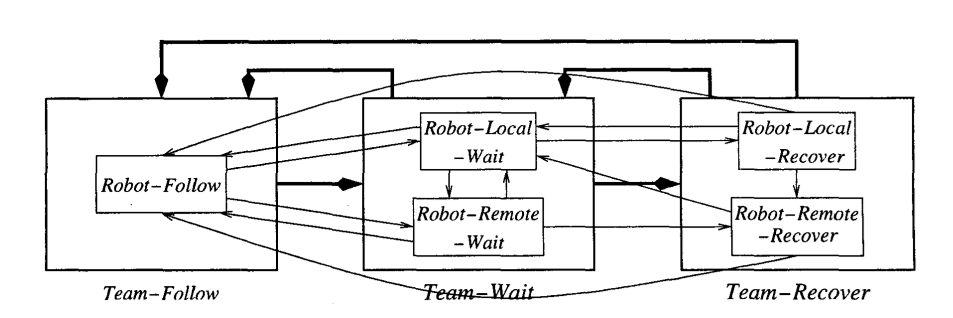
\includegraphics[width=1\textwidth]{figures/state_table_article1.png}
    \caption{State diagram for team and local behaviours}
    \label{fig:fig1}
\end{figure}

To enabe communication between the team global counters are used for wait and recovery states. Everytime a robot faces a dangerous situation both counters are increased and a timer starts, when the timer ends the wait counter decreases. Finally, when the danger is over the recovery counter is decreased too. These counters provide additional feedback to the other robots and enhance their sensorial information. If at some point a robot would fail in the middle of a dangerous situation the other robots have a timer that enabes them to sense that and resume operations after a certain time.
The software was executed with a group of 3 to 5 mobile patforms. Each one equiped with different sensors and with different characteristics.
Moreover, it was buit as a muti-threaded program, so each sensor has its own threat and then the output is sent to another threat which decides based on a set of fuzzy rules. The communication aso has its specific threat.
Finay, to recognise and track the eader a combination of CCD image sensor and aser scanner is used. The laser enabes the robot to sense the minimum distance and the CCD alows to detect the shape of the robot to follow with the following sequence:
\begin{enumerate}[1.-]
	\item \textbf{color segmentation:} searches a charachteristic coor of the robots.
	\item \textbf{Averaging (smoothing):} Depends on neightbours, if four or more are red, then red. Otherwise white.
	\item \textbf{Blob detection:} Examines regions by boundaries of red pixels.
	\item \textbf{Object assignment:} Diferent label for each connected component.
	\item \textbf{Object selection:} Decides which of the objects should be track by comparing the center of mass of every distinct object with the positon of the previous tracked robot.
	\item \textbf{Proximity estimation:} Depending on the size of the blob it estimates the distance to the leader
	
\end{enumerate}


\end{document}
